\section{Protótipo}

Com base nos dados levantados, no processo definido e levando em consideração
as recomendações da IN4, foi projetada uma planilha que controla os principais
aspectos da gerência de uma ordem de serviço.

A primeira planilha, apresentada na figura \ref{fig:prot_geral} mostra como
seria um formulário com as principais informações de uma OS. A preocupação aqui
foi a de garantir a rápida identificação da OS sem duplicar informações.

\begin{figure}[H]
  \centering
  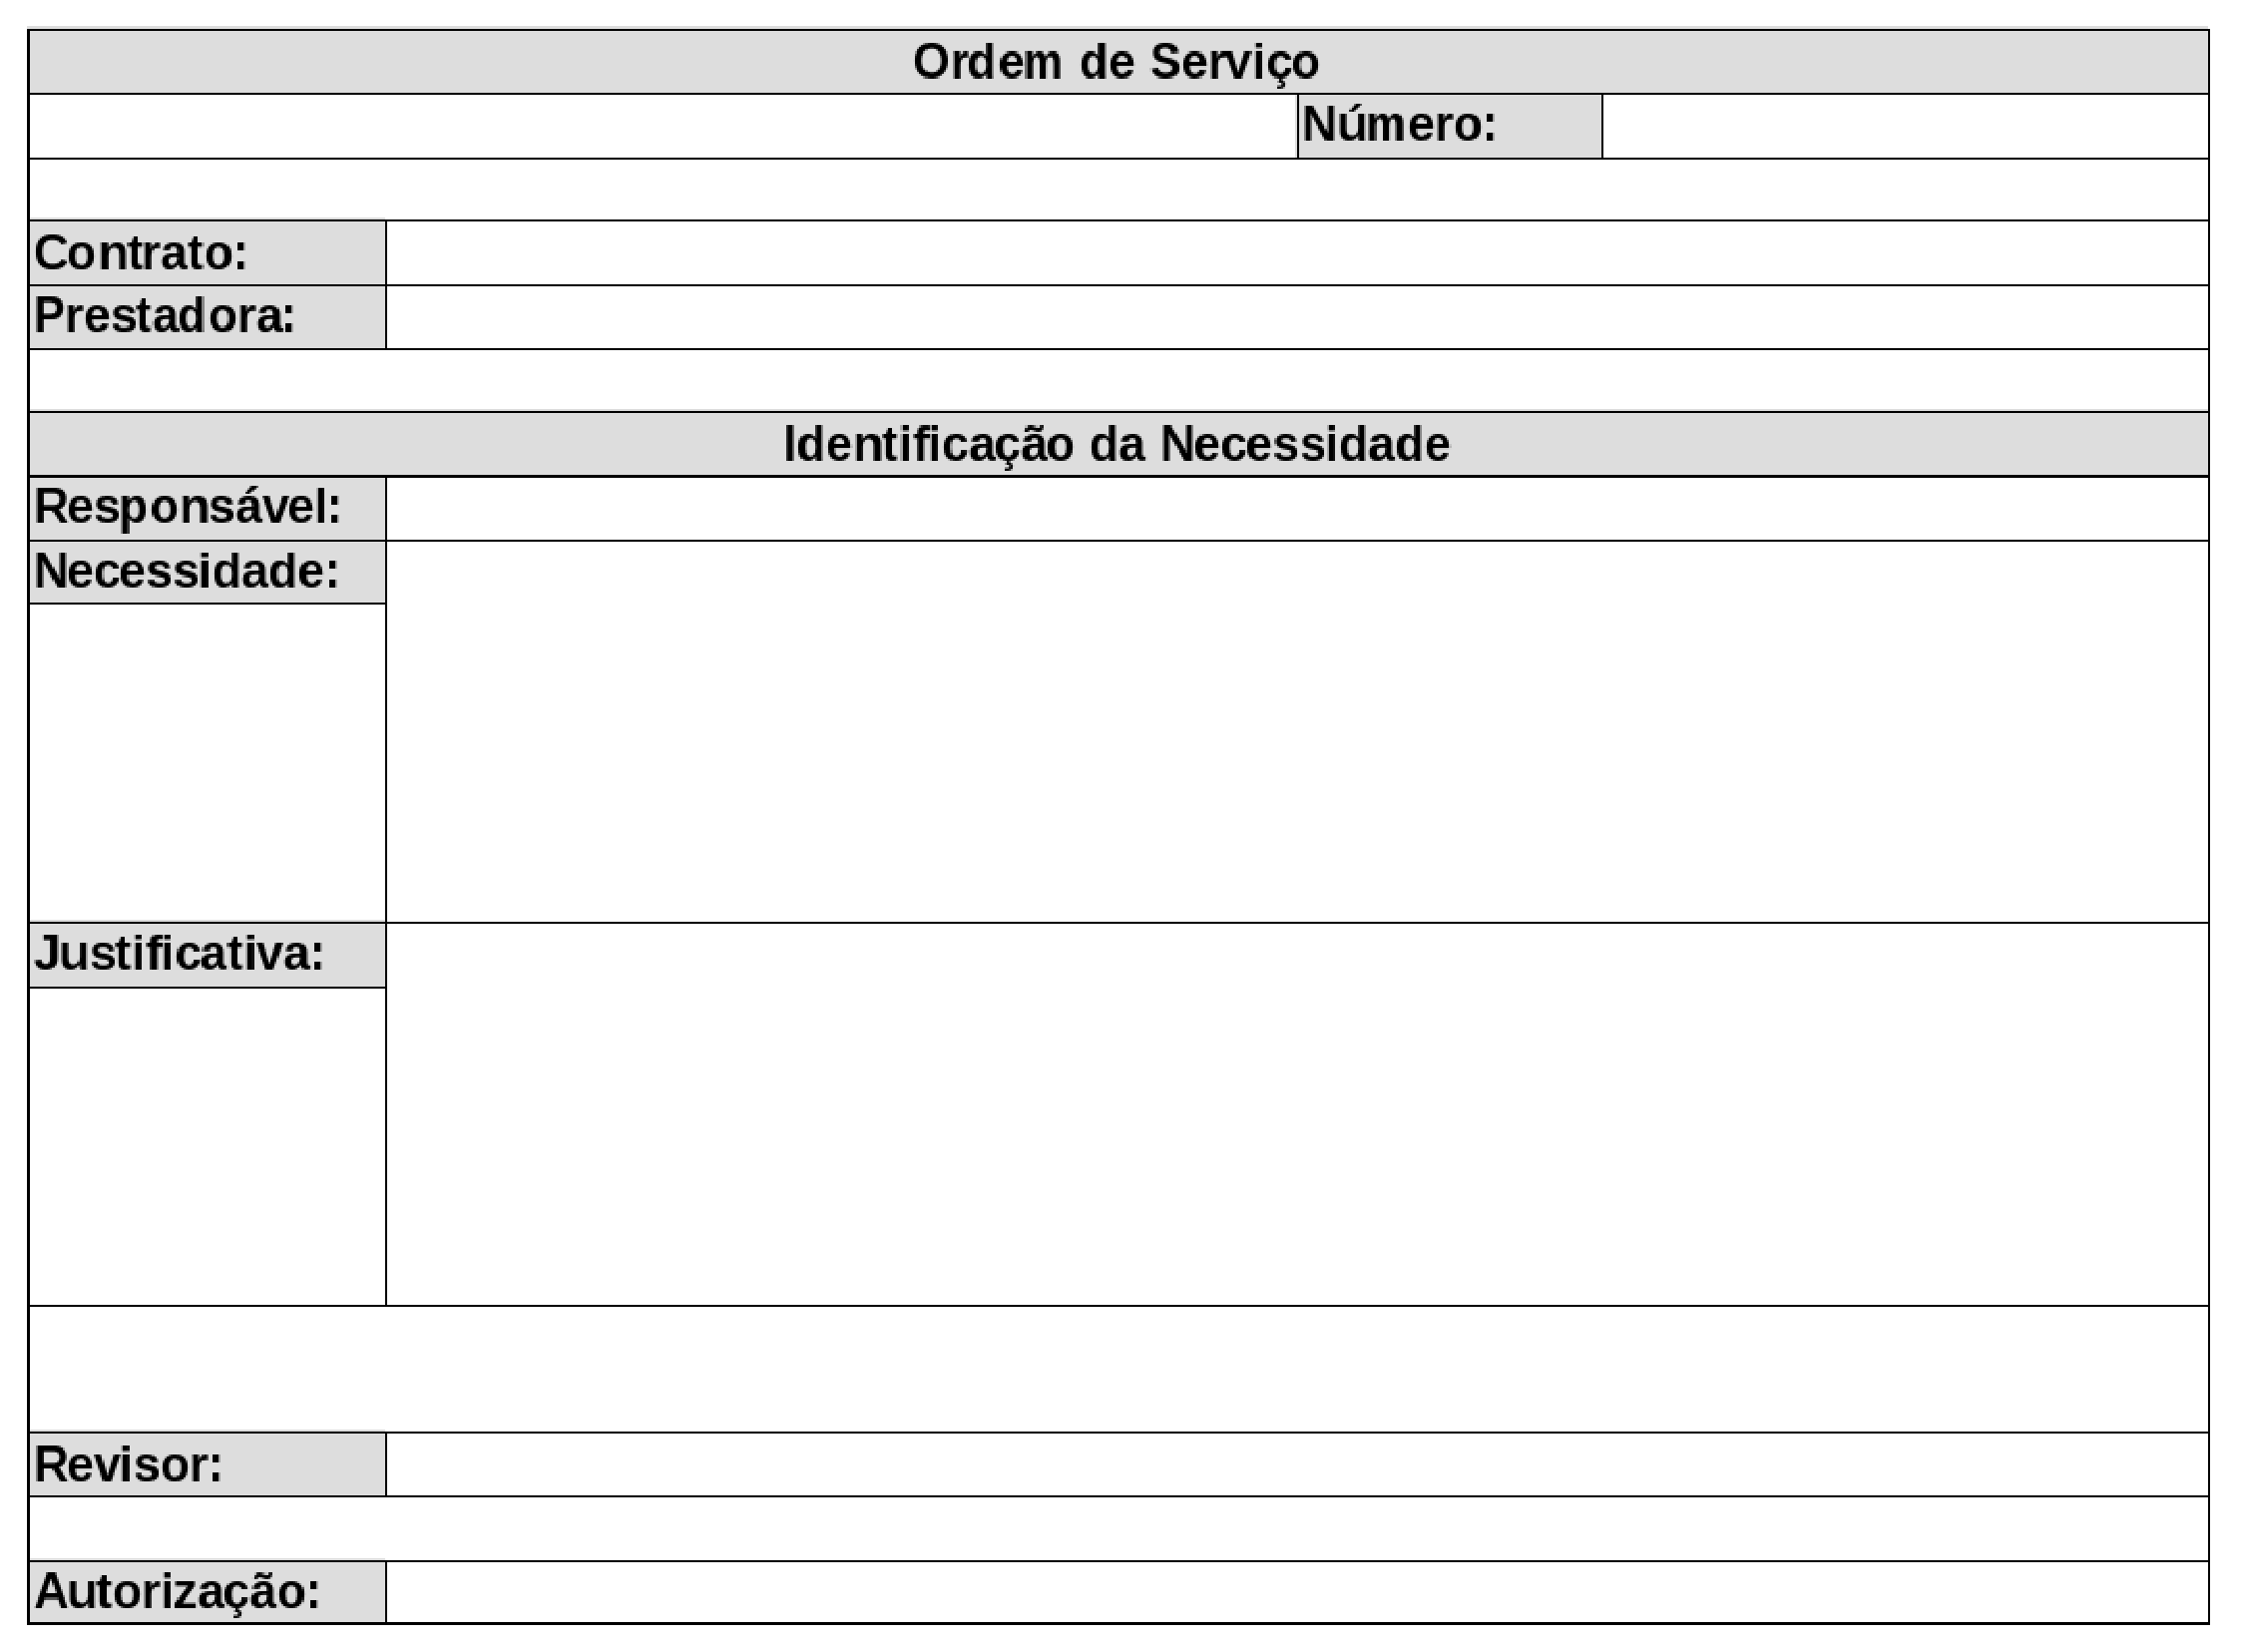
\includegraphics[keepaspectratio=true,scale=0.4]{figures/prot_geral}
  \caption{Identificação e justificativa de uma OS.}
  \label{fig:prot_geral}
\end{figure}

A segunda planilha, apresentada na figura \ref{fig:prot_itens} mostra como seria
o formulário dos itens de uma OS.

\begin{figure}[H]
  \centering
  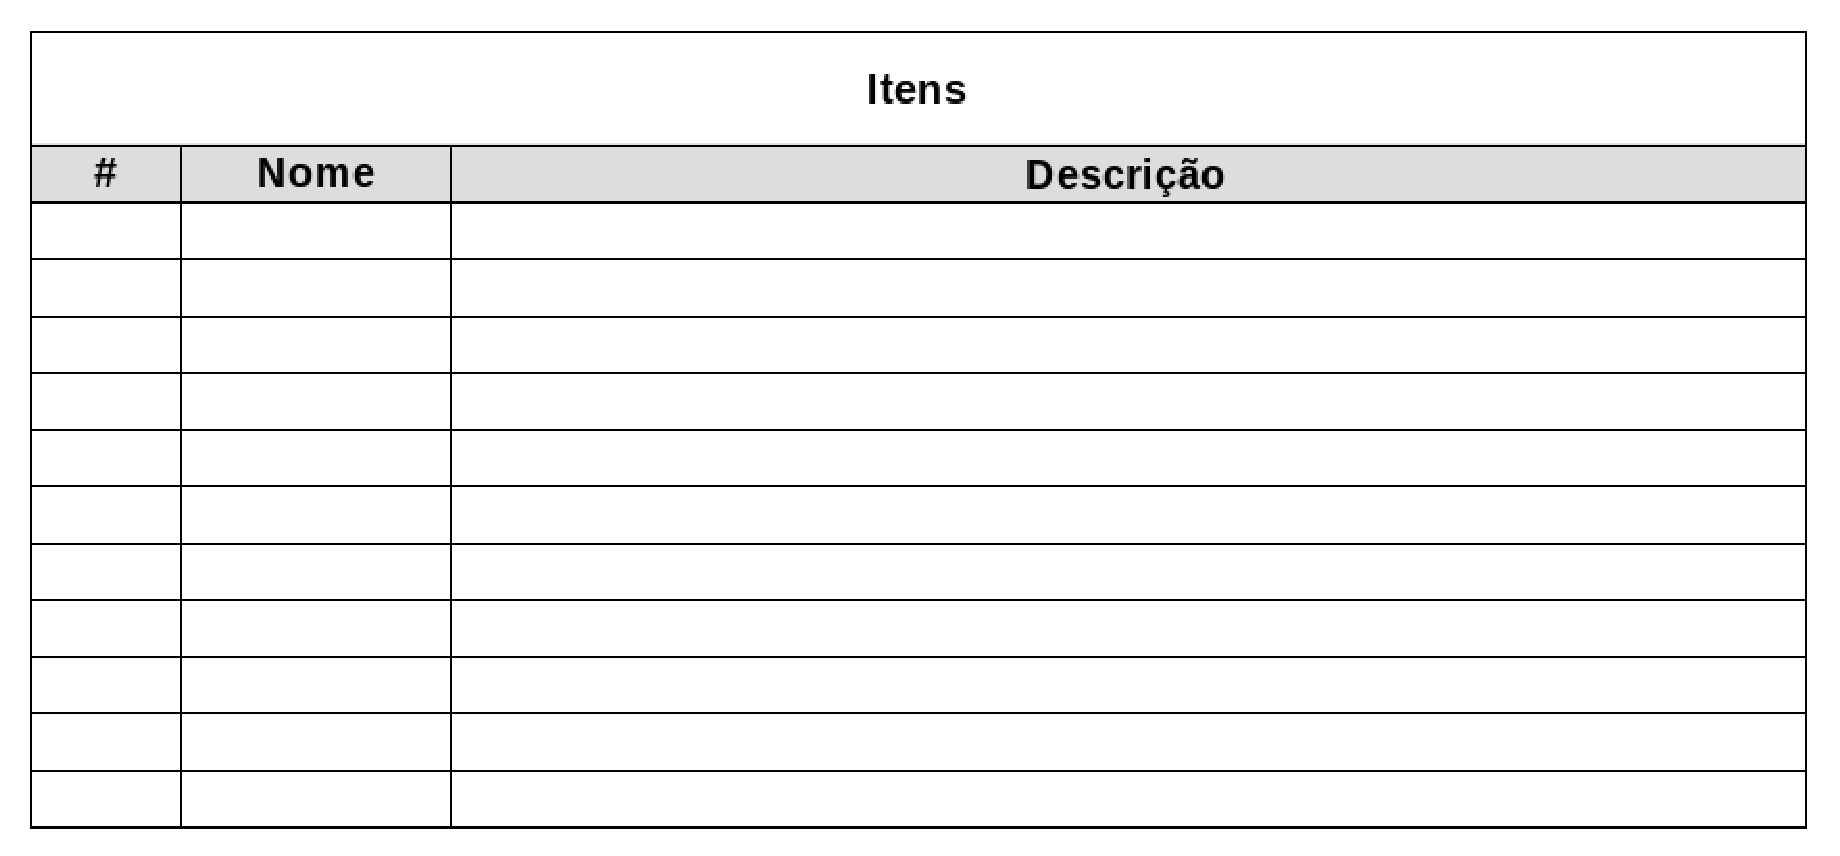
\includegraphics[keepaspectratio=true,scale=0.5]{figures/prot_itens}
  \caption{Itens de serviço a serem desenvolvidos pela Prestadora.}
  \label{fig:prot_itens}
\end{figure}

A terceira planilha, apresentada na figura \ref{fig:prot_eval} mostra como
seria um formulário com os critérios de avaliação dos itens de uma OS.

\begin{figure}[H]
  \centering
  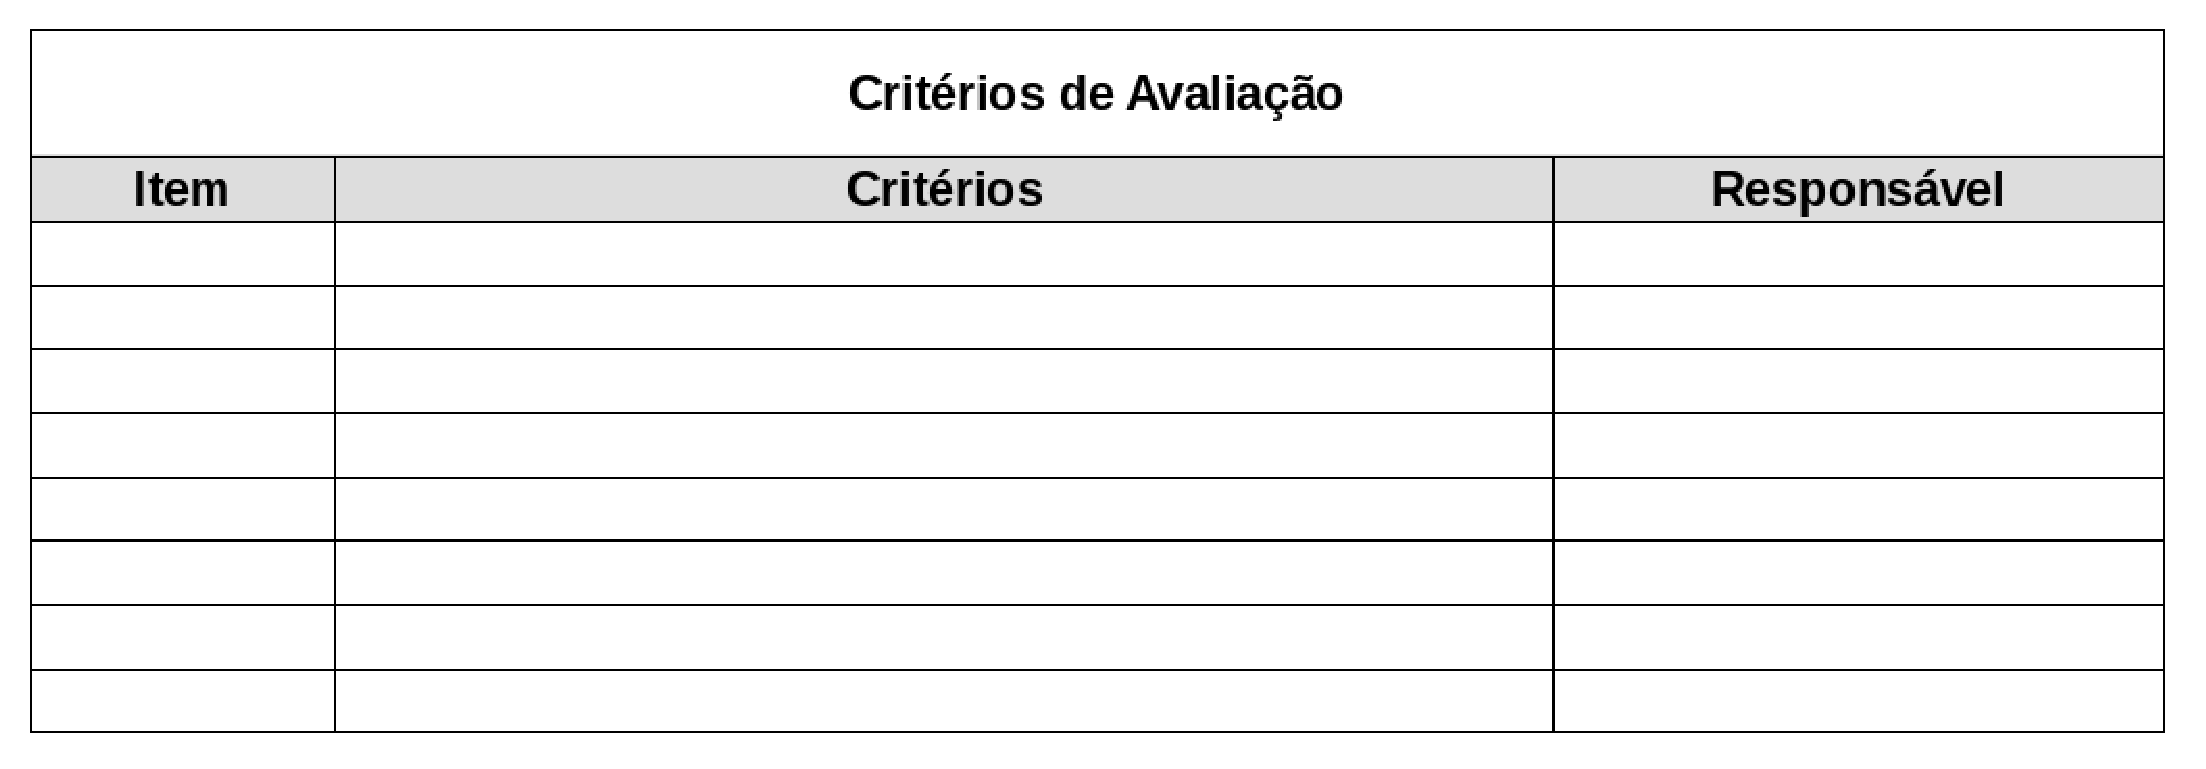
\includegraphics[keepaspectratio=true,scale=0.4]{figures/prot_eval}
  \caption{Critérios de avaliação acordados entre Contratante e Prestadora.}
  \label{fig:prot_eval}
\end{figure}

A quarta planilha, apresentada na figura \ref{fig:prot_ack_temp} mostra como
seria um formulário com o termo de recebimento provisório, que é entregue qundo
a Prestadora sinaliza que terminou o ciclo de desenvolvimento.

\begin{figure}[H]
  \centering
  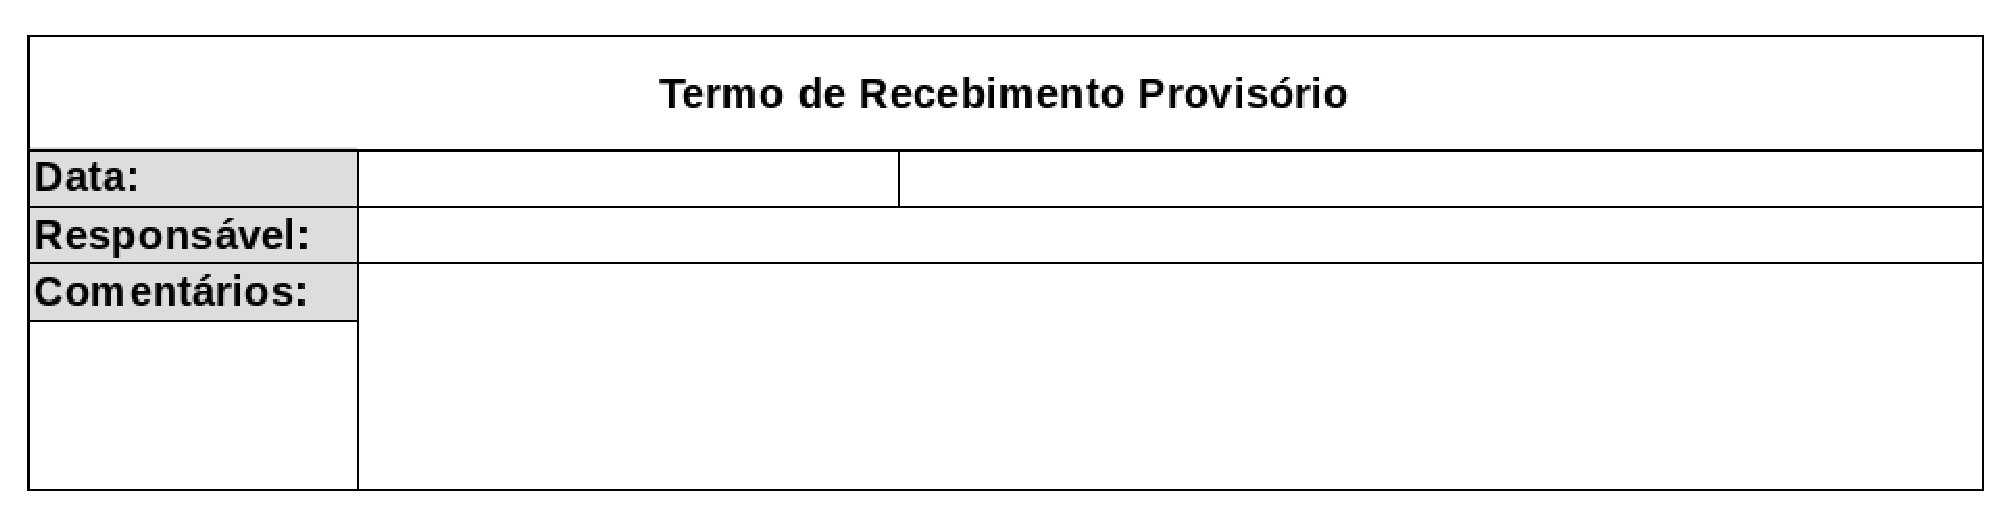
\includegraphics[keepaspectratio=true,scale=0.4]{figures/prot_ack_temp}
  \caption{Termo de Recebimento Provisório.}
  \label{fig:prot_ack_temp}
\end{figure}

A quinta planilha, apresentada na figura \ref{fig:prot_eval_report} mostra como
seria um formulário com o relatório de avaliação.

\begin{figure}[H]
  \centering
  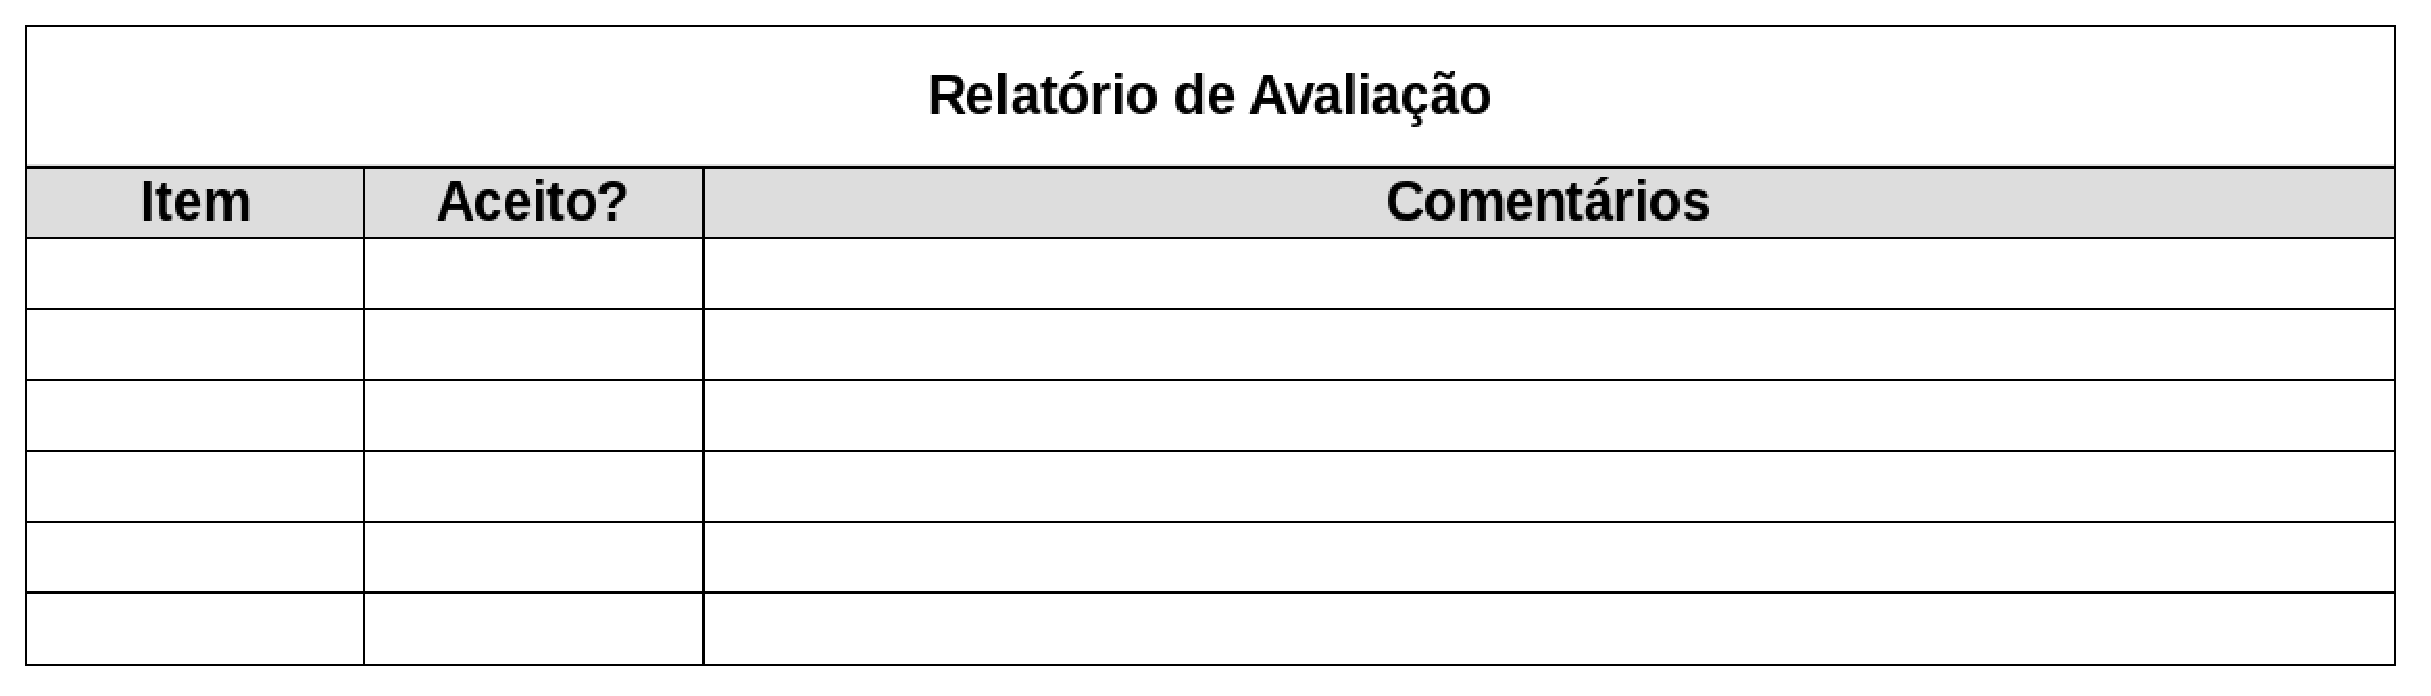
\includegraphics[keepaspectratio=true,scale=0.3]{figures/prot_eval_report}
  \caption{Relatório de Avaliação.}
  \label{fig:prot_eval_report}
\end{figure}

A sexta e última planilha, apresentada na figura \ref{fig:prot_ack} mostra como
seria um formulário com o termo de recebimento definitivo, que atesta que a
ordem de serviço foi concluída.

\begin{figure}[H]
  \centering
  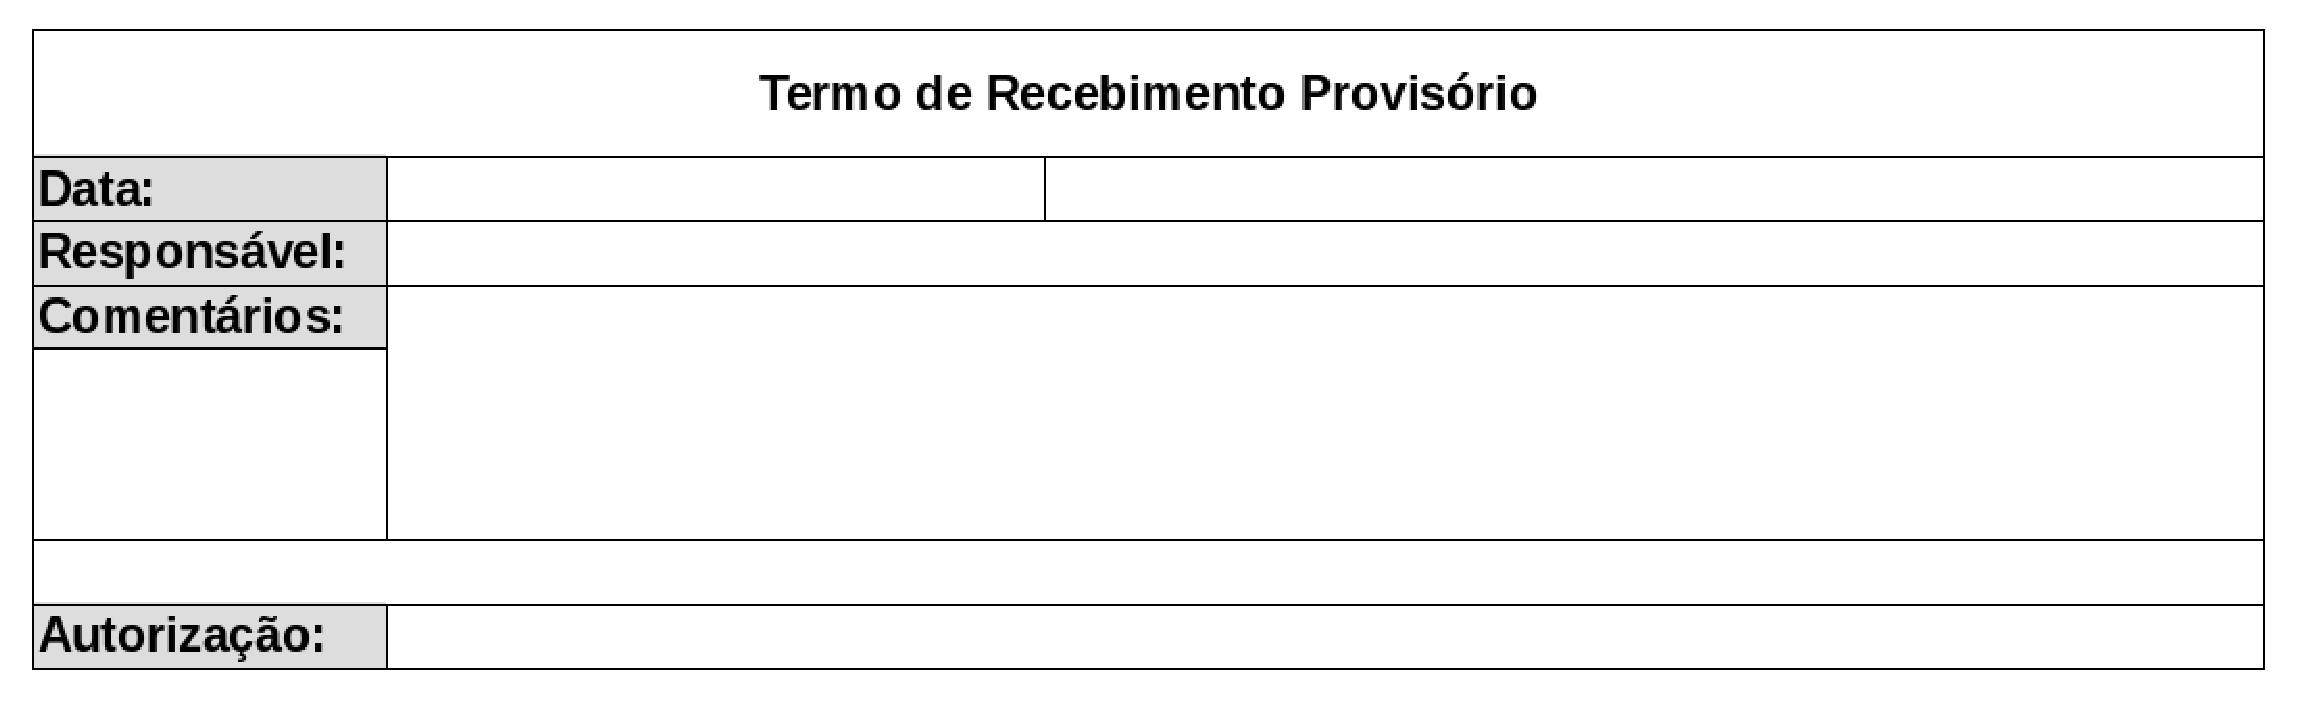
\includegraphics[keepaspectratio=true,scale=0.4]{figures/prot_ack}
  \caption{Termo de Recebimento Definitivo.}
  \label{fig:prot_ack}
\end{figure}
